This chapter presents an overview of the main works focused on the topics addressed in this dissertation.

\section{Related Works Description}
\label{s:RelatedWorks-Description}

The state-of-the art presents different computational techniques for data analysis. Lots of works found in the \ac{WWT} field use a combination of them to achieve their goal and improve the operation of the \acs{WWTP}s. Most of works aim to accomplish either faults detection, control, soft-sensing, variable prediction, or process understanding among others. Special attention will be given to the prediction task since it is the main focus of this investigation.
%either physical modelling, can have different purposes,

\ac{WWTP} are systems that exhibit a complex dynamic and require a high performance to accomplish the standards imposed by the environmental regulatory authorities \cite{Corominas2018}.  Considering the complex process nature, which presents a nonlinear behaviour and involves the interaction of physical, chemical, and biological components, results crucial the estimation and prediction of some key process variables. This enhance the control, process monitoring and simulation that increase the efficiency of the treatment  and the quality of the effluent \cite{Aalami2019,Arismendy2020,Liu2020}. Artificial intelligence methods are commonly used for solving the estimation and prediction challenges in nonlinear engineering science  problems \cite{Lotfi2019}. Literature introduces a wide landscape of strategies and techniques used to achieve mentioned task. \autoref{f:Techniques-Distribution} \cite{Corominas2018} shows the distribution of computational techniques used in the field of wastewater treatment for fault detection, prediction, soft-sensing, process understanding, control and optimization among others, it is made based on the number of papers published and cited in recent years. 

\begin{figure}[t]
\centering
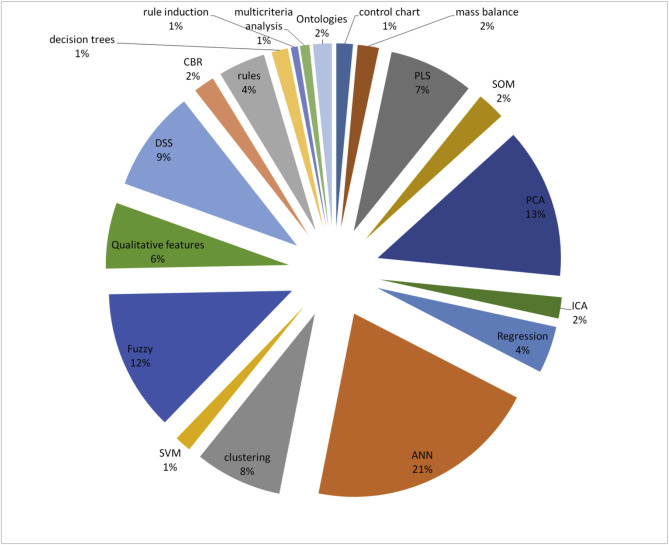
\includegraphics[width=15cm]{figures/3-Distribution-of-papers.jpg}
\caption{Techniques distribution \cite{Corominas2018}.}
\label{f:Techniques-Distribution}
\end{figure}

A research carried out by \cite{Corominas2018} shows that most of papers found make use of Artificial Neural Network (ANN), \ac{PCA} and \ac{FL} which are present in 46\% of the papers studied. Regarding the prediction tasks which is the focus of this work, Multiple Lineal Regression (MLR) models, FL, Partial Least Square (PLS), ANN and Support Vector Machines (SVM) are the main methods used where the last two stand out on nonlinear supervised learning. Other techniques involve in prediction are PCA, Self-organizing Maps (SOM), clustering, and Qualitative features commonly used for dimensionality reduction, information extraction, problem understanding, and variable selection.

One of the early approximations to intelligent monitoring and the predicting system was presented in \cite{Sanguesa2000} and \cite{Haggege2005}, where Bayesian networks and neuro-fuzzy logic were implemented to fulfill limitations of rule-based systems. Further works started to focus their attention on variable prediction using a variety of methods and a combination of them, taking the major advantages offered by each one. Reference \cite{Qin2012} used iterative predictor weighting–partial least squares (IPW–PLS) boosted by weighted predictions of a collection of regression models used as an ensemble prediction to estimate some water quality parameters. It was tested in the field, and its results showed a high correlation of the prediction. 

Several recent studies used fuzzy logic or neuro-fuzzy systems, such as \cite{Nourani2018,Nadiri2018,Han2018}, and some deep learning approaches, as in \cite{Guo2015,Alsina2018,Dairi2019}, which have provided high performance in prediction tasks. Studies like \cite{Bagheri2015} used a hybrid artificial neural networks–genetic algorithm approach to optimize the ANN estimation of the sludge bulking present in the sedimentation stage, which directly affects the effluent discharge water quality. Reference \cite{Dellana2009} made a performance comparison between the autoregressive integrated moving average (ARIMA) and time-delay neural network (TDNN) with such times-series variables as BOD and TSS and achieved more accurate predictions for real-world wastewater data with TDNN.

\section{Variable Prediction}
\label{s:RelatedWorks-variablePrediction}

\cite{Zhou2019} propose a set of decision-tree regression models to predict daily wastewater influent in two \ac{WWTP}s located in Ontario. Results for training and testing exhibit a \begin{math}R^2\end{math} of 0.97 and 0.72 for one facility and for the second one 0.96 and 0.58, respectively. \cite{Lu2020} evaluates the performance of two decision-tree based ensemble learners and enhances their performance with a data denoising technique called Complete Ensemble Empirical Mode Decomposition with Adaptive Noise (CEEMDAN) to predict Temperature, Dissolved oxygen, pH, Specific Conductance, and fluorescent dissolved organic matter. The enhanced Extreme Gradient Boosting (XGBoost) and Random Forest (RF) show the best results among other techniques used in the experiments, obtaining MAPEs from 0.27\% to 14.94\% in the best cases, depending on the variable selected to predict.

Study \cite{Alsulaili2021} implements a FFNN to predict the effluent BOD, COD and TSS in Kabd WWTP, Kuwait. The authors train the model with 1032 samples and take as input different influent parameters. This work presents a \begin{math}R^2\end{math} score of 0.75, 0.61 and 0.63, respectively. Also, \cite{Abba2017} determines the efficiency of ANN in predicting effluent COD of Nicosia WWTP, Chipre. Six different ANN models are trained where diverse model structures, input variables and epochs of training are considered. The best results obtained present a \begin{math}R^2\end{math} of 0.70 which is an improvement compared with the baseline they established using MLR and obtained \begin{math}R^2\end{math} of 0.34.

Work \cite{Niu2020} proposes a hybrid predictive model that uses Deep Belief Networks (DBN), a  structure specialized in regression tasks. A Genetic Algorithm optimizes the hyperparameters of the network achieving a MAPE of 4.34\% and \begin{math}R^2\end{math} of 0.6 for the effluent COD prediction.

Reference \cite{Zhao2021} compares the impact of the optimization algorithm used during the training of a FFNN implemented with the aim of predict effluent Total Nitrogen (TN). The baseline model uses backpropagation optimization algorithm and achieves a \begin{math}R^2\end{math} value of 0.85 and 0.26 for training (104 data points) and testing dataset (20 data points), respectively. The implementation of Levenberg-Marquardt (L-M), Bayesian Regularization (BR), and Scale Conjugate Gradient (SCG) optimization algorithms shows an improvement in the overfitting of the baseline model, obtaining \begin{math}R^2\end{math} of 0.88, 0.84, and 0.84 during training and 0.87, 0.78, and 0.86 over the whole set respectively.

Another example \cite{Manu2017} compares the performance of  SVMs and Adaptive Neuro-Fuzzy Inference Systems (ANFIS) in the prediction of discharge total Nitrogen concentration for the Kavoor WWTP located at Mangalore. ANFIS are fuzzy logic systems where the structure is replaced by neural network. Experiments show that SVMs overcome the results obtained by the ANFIS, achieving a \begin{math}R^2\end{math} of 0.82 versus 0.62 with Trapezoid Membership Functions and 0.72 with Gaussian Membership Functions. 

Work \cite{Guo2015} aims to predict one day interval TN concentration of effluent stream from Yong-yeon \ac{WWTP} in Ulsan, Korea. Measurements of some parameters from different points of the treatment serve as inputs for two Machine Learning models: ANN and SVM. Results show a \begin{math}R^2\end{math} for training and validation of 0.55 and 0.47 for the ANN and 1.00 and 0.46 for the SVM approach. Both models use 200 and 90 samples for training and validation process, respectively.

Recurrent neural networks are also used to in wastewater data-driven modelling. \cite{Yaqub2020} uses Long Short-Term Memory (LSTM) Neural Networks to predict removal efficiency of NH4-N, TN, and TP from a WWTP at Okcheon, Republic of Korea. A year of data with hourly frequency measurements constitute the dataset used for this work. A set of 5000 data points build the sequences of 10 previous observations used to train the LSTM model. The testing step shows the Mean Squared Error (MSE) values of 0.0047, 0.015, and 0.018 respectively, by using 1876 new data points. Study \cite{Kang2020} proposes a Bidirectional LSTM and compares the results with SVM, Gated Recurrent Unit (GRU) Neural Network, and standard LSTM. Experiments show that Bi-LSTM performs at least as well as other models and obtain better results in some scenarios.

A Generalized Regression Neural Network (GRNN) is implemented in \cite{Heddam2016}, a network architecture made of four layers: the input layer, the pattern layer, the summation layer, and the output one. This architecture offers a high performance in non-linear regression analysis, reason why it is used to estimate the effluent BOD based on other effluent parameters. Results are compared with a MLR showing that the GRNN performs better for the BOD estimation, achieving \begin{math}R^2\end{math} of 0.75 and 0.80 for training and testing, where 553 and 138 samples are respectively used. 

\cite{Baki2019} test the predictive capabilities of diverse regression models used to estimate the BOD in the Antalya Hurma WWTP. The study implements four different methods, classical regression analysis (CRA), Multivariate Adaptive Regression Splines (MARS), Artificial Bee Colony (ABC), and teaching learning-based optimization (TLBO). (Baki et al., 2019) uses 186 samples corresponding to 80\% of the available data to train all four proposed techniques, which yield \begin{math}R^2\end{math} values of 0.74, 0.79, 0.78, and 0.74 over the test dataset.

\cite{Guo2020} innovates in the use of Convolutional Neural Networks (CNN) together with Recurrent Neural Networks. The system proposed (PC-CR) uses a convolution layer, a pooling layer, and a fully connected layer as feature extractor, follow by an LSTM to achieve the COD and Ammonia Nitrogen prediction in the outlet of a sewage treatment plant located in Nan'an District, Chongqing, China.

Work \cite{Nourani2018} compares the performance of FFNN, ANFIS, SVR, and MLR models to predict COD, BOD, and TN at the Nicosia WWTP effluent stream. An averaging unit combines the output of the four models improving the final prediction up to 24\%. Three different ensemble techniques are implemented, all of them present R2 higher than 0.8 in validation. Another example of ensemble learner \cite{Nourani2021} utilizes FFNN, SVR, ANFIS, and ARIMA to predict COD and BOD effluent in Tabriz WWTP. Additional to the ensemble jittered data is used to enhance the model learning capabilities. Results show that both ensemble techniques and jittered data improved the system predictive performance where the ensemble jittering model exhibits \begin{math}R^2\end{math} of 0.85/0.86 (COD/BOD) in comparison with \begin{math}R^2\end{math} of 0.82/0.81 with the standard ensemble model.  

\section{Intelligent Control}
\label{s:RelatedWorks-Control}

Less common but also present in the state of the art, there are hybrid models that combine mechanistic, heuristic, and data-driven models. As an example, \cite{Hvala2020} improves the predictive performance of a mechanistic model based on the ASM2d model (Activated Sludge Model version 2d) using a Gaussian process technique increasing the \begin{math}R^2\end{math} value from 0.61 to 0.8 for effluent Total Nitrogen and from 0.54 to 0.65 for effluent total phosphorus.

In \cite{Pang2019}, a q-learning (QL) algorithm with an activated sludge model (ASM2d-guided) reward setting was proposed. The integrated ASM2d-QL algorithms equipped with a self-learning mechanism were derived for optimizing the control strategies (hydraulic retention time (HRT) and internal recycling ratio (IRR)) of the WWTP system. In reference \cite{Li2013}, a Bayesian network-based approach was proposed for real-time prediction of a wastewater treatment system based on Modified Sequencing Batch Reactor (MSBR) . Based on the framework of the modified sequencing batch reactor prediction analysis, a Bayesian network model was constructed to analyze an MSBR using training data and information provided by domain experts.

Work \cite{Haggege2005} is a synthesis of a new neuro-fuzzy controller with an online learning procedure and a simple algebraic formulation, making it easy to interpret by a human being to control a bioreactor without requiring any analytical representation. The authors in \cite{Nadiri2018} focused on the Tabriz \ac{WWTP}, proposing an ensemble of fuzzy logic (FL), committee fuzzy logic (CFL)  and supervised CFL to predict water quality parameters. In \cite{Nourani2018}, three nonlinear models (feedforward neural network, adaptive neuro-fuzzy interference system and support vector machines (SVMs)) and a classical multilinear regression (MLR) were applied to predict the performance of the Nicosia wastewater treatment plant in terms of biochemical oxygen demand (BOD), COD and total nitrogen (TN). 

In work \cite{Bagheri2015}, multilayer perceptron ANN–genetic algorithm (MLPANN–GA) and radial basis function ANN–genetic algorithm (RBFANN–GA) models were successfully implemented for sludge volume index (SVI) prediction, taking into account that when sludge bulking appears, it causes poor settleability of sludge that results in poor effluent quality, loss of active biomass and increased costs and poses several environmental hazards. BOD, COD, nitrate, ammonia, TN, total phosphorus (TP), total suspended solids (TSS), total dissolved solids (TDS), mixed liquor volatile suspended solids (MLVSS ), mixed liquor suspended solids (MLSS), SVI, dissolved oxygen (DO), pH and T (Celsius) were measured and used for the estimation. The study \cite{Raduly2007} performed a simulation of plant behavior over a wide range of influent disturbances. An artificial neural network (ANN) was trained on the available WWTP, comparing ANN and a mechanistic WWTP model’s performances.

The study \cite{Liukkonen2013} proposed the Kohonen self-organizing map (SOM), a useful tool for illustrating the prevailing states of a process and their evolution, monitoring the alteration of wastewater quality and alerting in case of unusual behavior, such as increasing concentrations of harmful discharge components. The method provided an advanced and efficient way of monitoring and visualizing many measurements conducted in wastewater treatment. Article \cite{Jimenez2015} emphasized the high potential of some promising techniques, such as spectral analysis, and discussed issues that could appear soon concerning control of anaerobic digestion (AD) processes. The authors in work \cite{Reis2017} provided a critical outlook of the evolution of industrial process monitoring (IPM) since its introduction almost 100 years ago. Several evolution trends that have been structuring IPM developments over this extended period were briefly referred to, with more focus on data-driven approaches.

Reference \cite{Ye2020} is a review of developments in artificial intelligence technologies for environmental pollution controls, including prediction of removal efficiency, evaluation of fuzzy logic to the control of the WWTP aerobic stage and AI-aided soft sensors for estimation of hard-to-measure variables. 

\section{Fault Detection}
\label{s:RelatedWorks-faultDetection}

There is a research branch whose aim is the opportune fault detection in very stringent processes, especially when it is part of the operational critical path where any unexpected event that occurs leads to a stagnation. Depending on the type of fault detection, the prediction of the problem can be focused on:
- The system’s ability to operate under some given circumstances.
- The time range in which equipment needs no maintenance and logistic support \cite{Alsina2018}.

Regarding system operability, faults and potential causes can be found before they occur by analyzing some patterns in \ac{WWTP} data. The data visualization is capable of showing patterns that are products of a possible anomaly, known as abnormal patterns. These are classified as isolated, sustained, transient and drift \cite{Newhart2019}. Each one provides a hint about a future fault. Thus, it is possible to get fault information by looking at data behavior. Reference \cite{Dairi2019} implemented data-driven unsupervised anomaly detection approaches based on deep learning methods and clustering algorithms. The aim was to monitor and detect anomaly conditions in \ac{WWTP} operations. The results showed its ability to detect the vast majority of abnormal events reported by the operator \cite{Dairi2019}. 

 Reference \cite{Alsina2018} showed how machine learning models obtained better prediction results concerning traditional methods when increasing the size of the time-to-failure datasets. Four diverse machine learning approaches were implemented: ANN, SVM, random forest (RF) and soft computing methods. The reference \cite{Dairi2019} presented a data-driven anomaly detection approach based on deep learning methods and clustering algorithms to monitor influent conditions of WWTP, which affect treatment unit states, ongoing process mechanisms and product qualities. These techniques were recurrent neural networks (RNNs) and the function to delineate complex distributions from restricted Boltzmann machines (RBM), with various classifiers.
 
 On the other hand, basic reliability analysis focuses on the prediction of the period in which equipment needs no support. This technique allows for finding a probability function R(t) to forecast the performance time of a component without failing until a given period t \cite{Alsina2018}. The work of \cite{Alsina2016} used an ANN to find the best cumulative failure distribution of mechanical components, which had a performance to fit a set of failure data and estimate its parameters, especially under poor data conditions. As a result, the networks with a momentum equal to 0.75 produced the best approximation 83.46\% of the time \cite{Alsina2016}.


\section{Soft-Sensing}
\label{s:Related-Works-SoftSensing}

Work \cite{Zounemat-Kermani2019} is a survey of the feasibility of utilizing soft computing models in predicting emission factors (gaseous H2S) based on five input parameters, namely, the total dissolved sulfides, biochemical oxygen demand (BOD5), temperature, flow rate and pH. Multivariate nonlinear autoregressive exogenous (NARX) neural networks were developed and applied to predict weekly H2S in four WWTPs. The paper \cite{Yu2019} described an optimized extreme learning machine (ELM) based on an improved cuckoo search (ICS) algorithm for the design of the soft BOD measurement model.

The study \cite{Hernandez-del-Olmo2019} performed different machine learning techniques to model a soft sensor to predict weather conditions such as SVMs, k-nearest neighbors (KNN), decision trees (DT), RFs and Gaussian naive Bayes (GND). With accurate weather prediction, an advanced control system can fit the parameters for better performance.

For paper \cite{Han2018}, a data-driven intelligent monitoring system was implemented (using the soft sensor technique and data distribution service). A fuzzy neural network (FNN) was applied for designing the soft sensor model.

\cite{Shen2018} compares the performance of four models; a multi-layer perceptron Neural Network trained with L-M algorithm, a backpropagation trained Neural Network, a Radial Basis Feed-forward neural network (RBNN), and a GRNN. All four model are trained with 410 samples representing the 75\% of the whole data and the results show that RBNN outperform the others obtaining a MAPE of 13.7\%/14.4\% and \begin{math}R^2\end{math} of 0.92/0.91 for training and validation, respectively.

Other research introduces the use of FL especially combined with another computational technique to enhance its performance. \cite{Huang2015} uses a neural fuzzy system combined with a Genetic Algorithm (GA) to estimate real-time nutrient concentrations in a biological stage of a wastewater treatment process. The GA-NFS soft-sensor estimates nitrogen and phosphorus concentration, and COD obtaining MAPEs of 16.18\%, 24.56\% and 7.8\% respectively. They encourage the addition of the GA component comparing this GA-NFS with a simple NFS, which obtained MAPEs of 31.86\%, 26.19\% and 22.79\% for each variable, demonstrating the impact of the optimization.

\section{Data Tools}
\label{s:Related-Works-Data-Tools}

Nowadays, since the world creates new data every single second, it has had to look for technologies to treat this data properly. In the market, some of them are Apache Hadoop and SciDB (open source) and others owned by supercompanies like Google, IBM, Amazon and Microsoft (frameworks) [32]. Each framework is specialized to do a particular task. A review [33] synthesized these frameworks as shown in Table 1 (adapted from [33]). Besides, the main languages for analytics, data mining and data science are R, SAS and Python. Each language has weaknesses and strengths. However, according to a Burtch Works poll (2019), computer scientists and engineers preferred using Python, as shown in Figure 1

\section{Summary}
\label{s:Related-Works-Summary}

The final section of each major chapter should summarize the chapter. In comparison to the chapter, the summary should be short ($\frac{1}{2}$ to $2$ pages is normal).

\begin{figure}[t]
\centering
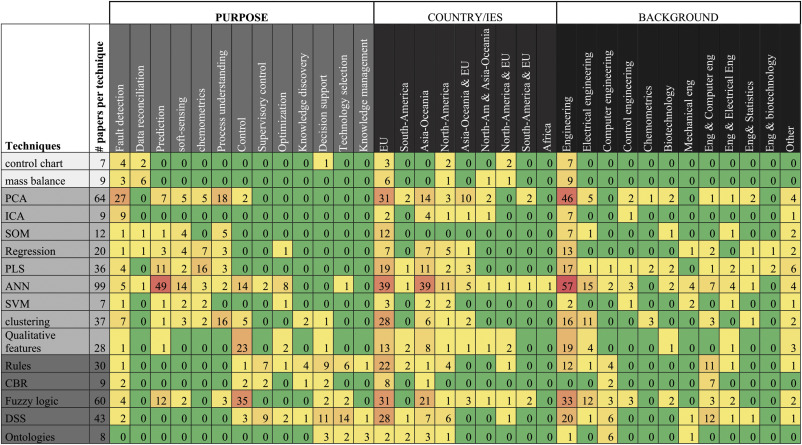
\includegraphics[width=16cm]{tables/PaperTable.jpg}
\caption{Number of papers per technique, for different purposes (only the main purpose of the method for each paper was considered), regions and background from the authors of the publications.}
\label{f:Papers Table}
\end{figure}
